% !TeX encoding = UTF-8
% !TeX spellcheck = pl_PL

% $Id:$

%Author: Wojciech Domski
%Szablon do ząłożeń projektowych, raportu i dokumentacji z steorwników robotów
%Wersja v.1.0.0
%


%% Konfiguracja:
\newcommand{\kurs}{Roboty Mobline}
\newcommand{\formakursu}{Projekt}

%odkomentuj właściwy typ projektu, a pozostałe zostaw zakomentowane
%\newcommand{\doctype}{Za\l{}o\.{z}enia projektowe} %etap I
\newcommand{\doctype}{Raport} %etap II
%\newcommand{\doctype}{Dokumentacja} %etap III

%wpisz nazwę projektu
\newcommand{\projectname}{Linefollower}

%wpisz akronim projektu
\newcommand{\acronim}{ABEKline}

%wpisz Imię i nazwisko oraz numer albumu
\newcommand{\osobaA}{Anna \textsc{Bernaś}, 241613}
%w przypadku projektu jednoosobowego usuń zawartość nowej komendy
\newcommand{\osobaB}{Emilia \textsc{Kalińska}, 241619}

%wpisz termin w formie, jak poniżej dzień, parzystość, godzina
\newcommand{\termin}{ptTN15}

%wpisz imię i nazwisko prowadzącego
\newcommand{\prowadzacy}{dr in\.{z}. Wojciech \textsc{Domski}}

\documentclass[10pt, a4paper]{article}

%Preambuła dokumentu

% linki w spisie tresci, bibliografi
\usepackage[bookmarks=true,bookmarksnumbered=false,unicode=true,pdftex=true, colorlinks,filecolor=black,linkcolor=black,urlcolor=black,citecolor=black]{hyperref}

%ustawienie rozmiaru papieru
\usepackage[a4paper, left=2.5cm, right=2.5cm, top=2.5cm, bottom=2.5cm, headsep=1.2cm]{geometry}

%rozmaite ustawienia pozwalające okreslić język

%NALEŻY wybrać jeden z pakietów
%\usepackage{polski} %przydatne podczas składania dokumentów w j. polskim
\usepackage[polish]{babel}  % pakiet lokalizujący dokument w języku polskim
%\usepackage[british]{babel}

\usepackage{indentfirst}	% polski styl pisania (np. rozpoczecie pierwszego akapitu
% pod nazwa rozdzialu od wciecia)
%\usepackage[OT4]{fontenc}
\usepackage[utf8]{inputenc} % w miejsce utf8 można wpisać latin2 bądź cp1250,
% w zależności od tego w jaki sposób kodowane są 
% polskie znaki diakrytyczne przy wprowadzaniu 
% z klawiatury.
%kodowanie znaków, zależne od systemu
\usepackage[T1]{fontenc} %poprawne składanie polskich czcionek

%OPEROWANIE NA OBRAZACH
\usepackage{graphicx}       % pakiet graficzny, umożliwiający m.in.
% import grafik w formacie eps
%\usepackage{epstopdf}		% pozwala na importowanie grafik w formacie eps
% przy użyciu pdflatex
\usepackage[update,prepend]{epstopdf}
\usepackage{rotating}       % pakiet umożliwiający obracanie rysunków
\usepackage{subfigure}      % pakiet umożliwiający tworzenie podrysunków
\usepackage{epic}           % pakiet umożliwiający rysowanie w środowisku latex
\usepackage{psfrag}         % pakiet umożliwiający podmianę łańcuchów znaków 
% w plikach eps
%\usepackage{curves}         % pakiet do wykreslania krzywych

%pakiety dodające dużo dodatkowych poleceń matematycznych
\usepackage{amsfonts}       % pakiet z rozmaitymi czcionkami matematycznymi
%\usepackage{amssymb}        % pakiet z rozmaitymi symbolami matematycznymi
\usepackage{amsmath}        % pakiet z rozmaitymi środowiskami matematycznymi

\usepackage{fp}             % pakiet z funkcjami operujacymi 
% na liczbach zmiennoprzecinkowych
\usepackage{calc}           % pakiet umożliwiający operacje arytmetyczne
% na tzw. licznikach (liczbach całkowitych)
\usepackage{leftidx}		% indeksy górne i dolne po lewej stronie

%definicje matematyczne
\providecommand{\abs}[1]{\lvert#1\rvert}
\providecommand{\norm}[1]{\lVert#1\rVert}

%pakiety wspomagające i poprawiające składanie tabel
\usepackage{supertabular}
\usepackage{array}
\usepackage{tabularx}
\usepackage{hhline}
\usepackage{longtable}		% wsparcie dla dlugich tabel
\usepackage{multicol}		% podzial strony na wiele kolumn

%pakiet do BibTex
\usepackage{cite}

\usepackage{url} %pakiet pozawalający na dodawanie adresów url w bibliografi

%pakiet wypisujący na marginesie etykiety równań i rysunków zdefiniowanych przez \label{}, chcąc wygenerować finalną wersję dokumentu wystarczy usunąć poniższą linię
%\usepackage{showlabels}

\usepackage{float}			% lepsza obsluga mechanizmow obiektow plywajacych
% wymuszenie wstawienia np. tabeli, obrazka w danym miejscu przez [H]

\usepackage{listings}       % pakiet dedykowany zrodlom programow
\usepackage{color}


\definecolor{dkgreen}{rgb}{0,0.6,0}
\definecolor{gray}{rgb}{0.5,0.5,0.5}
\definecolor{mauve}{rgb}{0.58,0,0.82}

\lstset{ %
	language=C,                % the language of the code
	basicstyle=\small,           % the size of the fonts that are used for the code
	numbers=left,                   % where to put the line-numbers
	numberstyle=\footnotesize\color{gray},  % the style that is used for the line-numbers
	stepnumber=1,                   % the step between two line-numbers. If it's 1, each line 
	% will be numbered
	numbersep=5pt,                  % how far the line-numbers are from the code
	backgroundcolor=\color{white},      % choose the background color. You must add \usepackage{color}
	showspaces=false,               % show spaces adding particular underscores
	showstringspaces=false,         % underline spaces within strings
	showtabs=false,                 % show tabs within strings adding particular underscores
	%frame=single,                   % adds a frame around the code
	rulecolor=\color{black},        % if not set, the frame-color may be changed on line-breaks within not-black text (e.g. comments (green here))
	tabsize=2,                      % sets default tabsize to 2 spaces
	captionpos=b,                   % sets the caption-position to bottom
	breaklines=true,                % sets automatic line breaking
	breakatwhitespace=false,        % sets if automatic breaks should only happen at whitespace
	%title=\lstname,                   % show the filename of files included with \lstinputlisting;
	% also try caption instead of title
	keywordstyle=\color{blue},          % keyword style
	commentstyle=\color{dkgreen},       % comment style
	stringstyle=\color{mauve},         % string literal style
	escapeinside={\%*}{*)},            % if you want to add LaTeX within your code
	morekeywords={*,...},              % if you want to add more keywords to the set
	deletekeywords={...}              % if you want to delete keywords from the given language
}

%polish signs in lst code
\lstset{literate=%
	{ą}{{\k{a}}}1
	{ć}{{\'c}}1
	{ę}{{\k{e}}}1
	{ł}{{\l}}1
	{ń}{{\'n}}1
	{ó}{{\'o}}1
	{ś}{{\'s}}1
	{ż}{{\.z}}1
	{ź}{{\'z}}1
	{Ą}{{\k{A}}}1
	{Ć}{{\'C}}1
	{Ę}{{\k{E}}}1
	{Ł}{{\L}}1
	{Ń}{{\'N}}1
	{Ó}{{\'O}}1
	{Ś}{{\'S}}1
	{Ż}{{\.Z}}1
	{Ź}{{\'Z}}1
}

\usepackage{verbatim}       % pakiet dedykowany rozmaitym wydrukom tekstowym
\usepackage{ifthen}         % pakiet umożliwiający tworzenie prostych programów
% (m.in. zawiera instrukcje powtórzeniowe 
% i warunkowe)
\usepackage{upquote}		%normal quotations marks ' and `

% deklaracje wymagane przez pakiet theorem automatycznie ladowany w przypadku
% klasy dokumentu article
%
\newtheorem{Dn}{Definicja}[section]     % deklaracja srodowiska definicja
\newtheorem{La}[Dn]{Lemat}                % deklaracja srodowiska lemat
\newtheorem{Tm}[Dn]{Twierdzenie}          % deklaracja srodowiska twierdzenie
\newtheorem{Rk}[Dn]{Spostrze{\.z}enie}  % deklaracja srodowiska spostrzezenie
\newtheorem{Am}[Dn]{Algorytm}           % deklaracja srodowiska algorytm
\newtheorem{As}[Dn]{Za{\l}o{\.z}enie}   % deklaracja srodowiska zalozenie
\newtheorem{Pn}[Dn]{Propozycja}           % deklaracja srodowiska propozycja
\newtheorem{Py}[Dn]{W{\l}asno{\'s}{\'c}}  % deklaracja srodowiska wlasnosc
\newtheorem{Cy}[Dn]{Wniosek}              % deklaracja srodowiska wniosek
\newtheorem{Ee}[Dn]{Przyk{\l}ad}        % deklaracja srodowiska przyklad
\newtheorem{Ex}{{\'C}wiczenie}          % deklaracja srodowiska cwiczenie

%helps to specify width of a column in table
%\begin{tabular}{|C{1cm}|c|c|c|c|c|c|c|c|c|c|}
%first column will have widht of 1cm
\newcolumntype{L}[1]{>{\raggedright\let\newline\\\arraybackslash\hspace{0pt}}m{#1}}
\newcolumntype{C}[1]{>{\centering\let\newline\\\arraybackslash\hspace{0pt}}m{#1}}
\newcolumntype{R}[1]{>{\raggedleft\let\newline\\\arraybackslash\hspace{0pt}}m{#1}}

\sloppy			%zawija bardzo długie linie

\usepackage{pdfpages}
%\pagenumbering{gobble}% Remove page numbers (and reset to 1)
	
\begin{document}

\def\tablename{Tabela}	%zmienienie nazwy tabel z Tablica na Tabela

\begin{titlepage}
	\begin{center}
		\textsc{\LARGE \formakursu}\\[1cm]		
		\textsc{\Large \kurs}\\[0.5cm]		
		\rule{\textwidth}{0.08cm}\\[0.4cm]
		{\huge \bfseries \doctype}\\[1cm]
		{\huge \bfseries \projectname}\\[0.5cm]
		{\huge \bfseries \acronim}\\[0.4cm]
		\rule{\textwidth}{0.08cm}\\[1cm]
		
		\begin{flushright} \large
		\emph{Skład grupy:}\\
		\osobaA\\
		\osobaB\\[0.4cm]
		
		\emph{Termin: }\termin\\[0.4cm]

		\emph{Prowadzący:} \\
		\prowadzacy \\
		
		\end{flushright}
		
		\vfill
		
		{\large \today}
	\end{center}	
\end{titlepage}
\newpage
\tableofcontents
\newpage

%Obecne we wszystkich dokumentach
\section{Opis projektu}
\label{sec:OpisProjektu}

Celem projektu jest zbudowanie robota typu linefollwer tzn. robota mobilnego, który porusza się po wyznaczonej ścieżce. Zasada działania takiego robota polega na tym, że zadana trasa (czarna linia na białym podłożu) jest oświetlana przez diodę znajdującą się na przodzie robota (dioda emituje światło widzialne lub IR). Następnie za pomocą czujników jest sprawdzane w jakim stopniu jest odbijane światło od podłoża. Następnie za pomocą danych uzyskanych z czujników zostanie dokonana analiza położenia robota i nastąpi odpowiednie skorygowanie kierunku ruchu dobierając odpowiedni napęd dla poszczególnych kół. Rozszerzeniem projektu będzie umieszczenie na przedzie pojazdu czujnika, który będzie informował o przeszkodzie. W przypadku wykrycia przeszkody pojazd zostanie zatrzymany. Awaryjne zatrzymanie robota będzie odbywało się za pomocą komunikacji z wykorzystaniem modułu Wi-Fi. Wyżej opisana zasada działania jest zaprezentowana za pomocą schematu blokowego na rysunku \ref{fig:schematBlokowy}, natomiast architektura systemu została przedstawiona na rysunku \ref{fig:Architektura}. \\ \\
Podczas wykonywania projektu należy zwrócić uwagę na:
\begin{itemize}
    \item odpowiedni dobór silnika
    \item rozkład ciężkości robota
    \item sposób ułożenia czujników
    \item sposób zasilania
    \item implementację regulatora PID
\end{itemize}

\subsection{Założenia projektowe}

\begin{itemize}
    \item Logika oparta na Arduino.
    \item Napęd na dwa koła.
    \item Wykorzystanie aplikacji Blynk do zdalnego wyłączania robota za pomocą modułu WiFi.
    \item Zatrzymanie robota przed przeszkodą na podstawie odczytów z czujnika ultradźwiękowego.
    \itemŚledzenie czarnej ścieżki na białym podłożu za pomocą czujników odbiciowych.
\end{itemize}
\newpage
\begin{figure}[H]
	\centering
	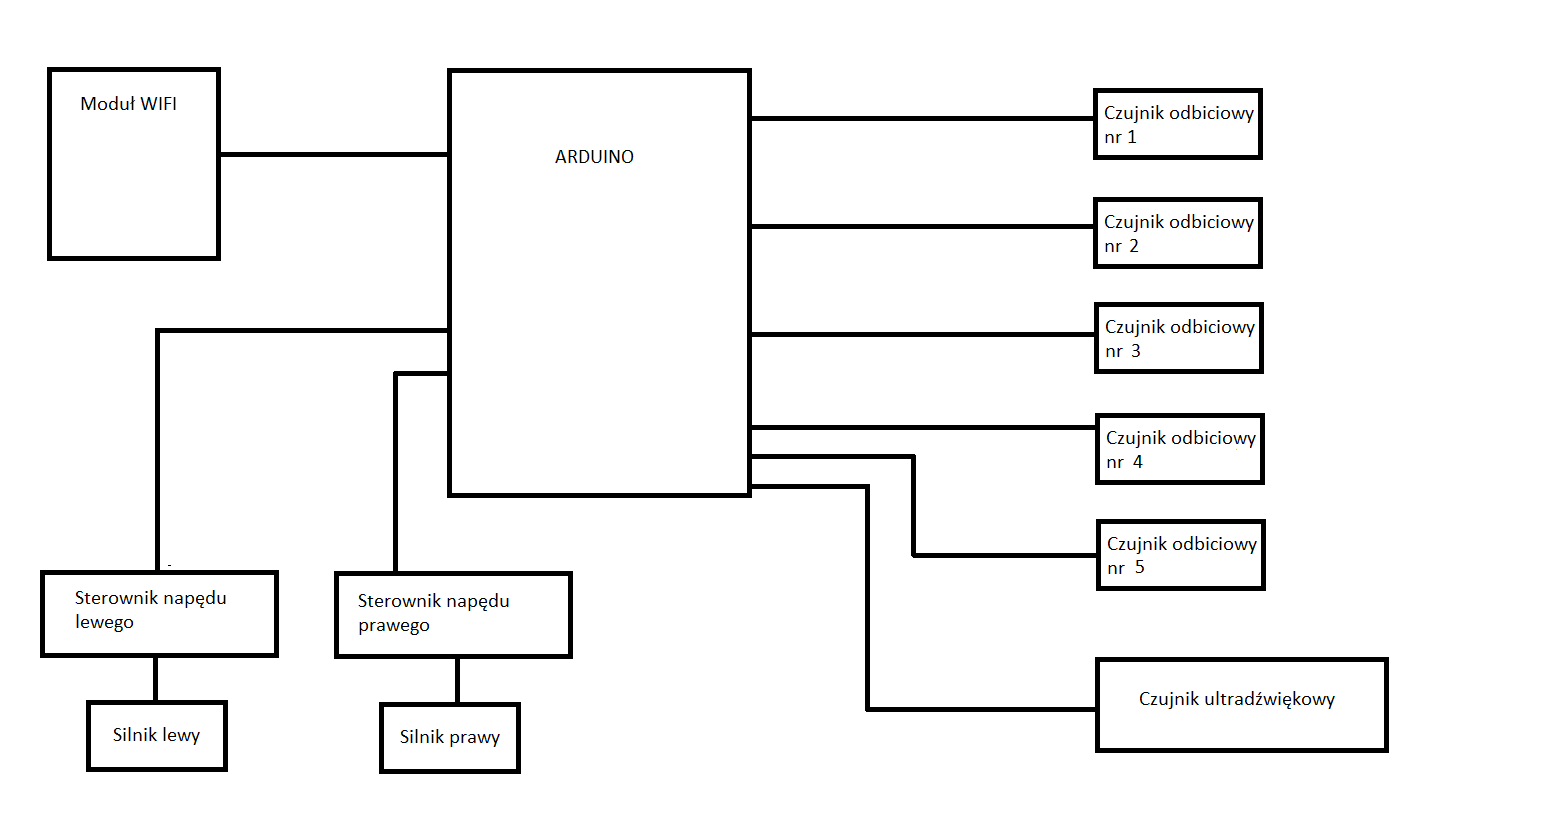
\includegraphics[width=\textwidth]{figures/Architektura.png}
	\caption{Architektura systemu}
	\label{fig:Architektura}
\end{figure}

\begin{figure}[H]
	\centering
	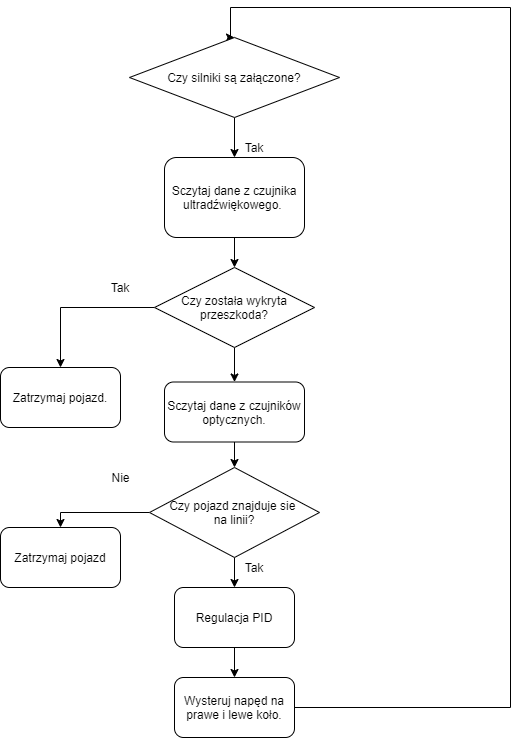
\includegraphics[width=0.5\textwidth]{figures/Linefollower.png}
	\caption{Schemat blokowy algorytmu sterowania}
	\label{fig:schematBlokowy}
\end{figure}
\newpage
%Obecne we wszystkich dokumentach
\section{Konfiguracja mikrokontrolera}


Konfiguracje zostały wykonane bazując na dokumentacjach Arduino \cite{dok1} oraz modułu Wi-Fi \cite{dok2}.


%Obecne we wszystkich dokumentach
\subsection{Konfiguracja pinów}

\begin{table}[H]
	\centering
	\begin{tabular}{|l|l|l|}
		\hline
		Numer pinu	&	PIN & Funkcja/etykieta\\
		\hline
		2&	3V3 & Wyjście regulatora 3.3V\\
		3&	AREF & Napięcie odniesienia\\
		4&	A0 & ADC0 - odczyt analogowy\\
		5&	A1 & ADC1 - odczyt analogowy\\
		6&	A2 & ADC2 - odczyt analogowy\\
		7&	A3 & ADC3 - odczyt analogowy\\
		10&	A6 & ADC6 - odczyt analogowy\\
		11&	A7 & ADC7 - odczyt analogowy \\
		14&	GND&  \\
		15&	VIN&   Zasilanie \\
		16&	TX1&    UART - WIFI\\
		17&	RX0&	UART - WIFI\\
		19&	GND&	\\
		20&	D2& Wyjście GPIO	\\
		21&	D3&	Wejście GPIO\\
		23&	D5&	PWM\\
		24&	D6&	PWM\\
		25&	D7&	Wyjście GPIO\\
		26&	D8&	Wyjście GPIO\\
		27&	D9&	Wyjście GPIO\\
		28&	D10&	Wyjście GPIO\\
	
		\hline
	\end{tabular}
	\caption{Konfiguracja pinów mikrokontrolera}
	
\end{table}

%Obecne we wszystkich dokumentach
\subsection{UART}

Interfejs szeregowy wykorzystywany będzie do komunikacji z modułem WIFI
ESP8266. Odbierane będą sygnały sterujące, a wysyłane dane odbierane z czujników oraz informacje o obecnym stanie robota.

\begin{table}[H]
	\centering
	\begin{tabular}{|l|c|} \hline
		\textbf{Parametr} & Wartość \\
		\hline
		\hline  \textbf{Baud Rate}&115200  \\\hline
		\textbf{Word Length } & 8 Bits \\\hline
		\textbf{Parity} &  None\\
		\hline
		\textbf{Stop Bits}& 1\\
		\hline
	\end{tabular}
	\caption{Konfiguracja peryferium UART}
	\label{tab:UART}
\end{table}

\subsection{ADC}

Przetwornik będzie służył do odczytu wielkości analogowych z czujników odbiciowych a także do pomiaru napięcia zasilania, a tym samym wskazania poziomu naładowania zasilania.

\begin{table}[H]
	\centering
	\begin{tabular}{|l|c|} \hline
		\textbf{Parametr} & Wartość \\
		\hline
		\hline  \textbf{Resolution}&10 Bits  \\\hline
		\textbf{ADC Clock } & 16 MHz \\\hline
		\textbf{Prescaler} &  128\\
		\hline
		\textbf{Conversion}& 13 ADC Clocks\\
		\hline
		\textbf{Sample Rate}& 9600 Hz\\
		\hline
	\end{tabular}
	\caption{Konfiguracja peryferium ADC}
	\label{tab:USART}
\end{table}

\subsection{PWM}

Sygnał z modulowaną szerokością impulsów posłuży do ustawiania szybkości obrotowej silników.

\begin{table}[H]
	\centering
	\begin{tabular}{|l|c|} \hline
		\textbf{Parametr} & Wartość \\
		\hline
		\hline  \textbf{Base Frequency}&62500  \\\hline
		\textbf{Prescaler} &  1\\\hline
		
	\end{tabular}
	\caption{Konfiguracja peryferium PWM}
	\label{tab:USART}
\end{table}


%sama uznalam ze jest potrzebny taki rozdzial
\section{Wybrane komponenty}
\begin{itemize}
    \item Czujnik transoptor odbiciowy CNY70 \cite{dok4}.
    \item Ultradźwiękowy czujnik odległości HC-SR04 \cite{dok3}.
    \item Moduł WiFi ESP-01 ESP8266 \cite{dok2}.
    \item Arduino Nano Every - ABX00028 \cite{dok1}.
    \item Dwukanałowy sterownik silników L293D \cite{dok5}.
    \item Silniki N20-BT01 micro 75:1 220RPM Pololu \cite{dok6}.
    \item Akumulator Li-Pol Dualsky 11.1V 400mAh 35C.
\end{itemize}



%Obecne w dokumencie do etapu II oraz III
\section{Projekt elektroniki}


Robot posiada dwa niezależne napędy umieszczone na jednej osi. Każdy z nich jest realizowany przez silnik DC z przekładnią. Sterowanie silników odbywa się poprzez zastosowanie dwukanałowych sterowników. Prędkość obrotowa wału definiowana będzie za pomocą sygnału PWM, natomiast kierunek obrotu za pomocą dwóch linii dwustanowych. Sterowanie silnikami będzie możliwe dzięki głównemu sterowników pokładowemu, którym jest Arduino. Zasilanie części logicznej sterownika będzie zapewnione dzięki podaniu napięcia zewnętrznego z akumulatorów na wewnętrzny regulator. Sterownik za pomocą przetworników ADC będzie pobierać wartości analogowe uzyskane z pięciu czujników odbiciowych (detektorów linii czarnych). Odczyt z czujnika ultradźwiękowego będzie możliwy dzięki linii wyzwalania i linii informacji zwrotnej. Zasilanie czujników (5V) zapewniane będzie przez przetwornice, tak samo jak zasilanie części logicznej sterowników silników. Dzięki akwizycji danych z czujników możliwe jest wysyłanie o aktualnym stanie robota przez interfejs szeregowy UART do modułu WiFi. Moduł WiFi będzie pracować na logice 3,3V, dlatego linie TX i RX zostały poddane konwersji poziomów za pomocą konwertera zrealizowanego na tranzystorze MOSFET oraz moduł zasilany będzie z przetwornicy napięciem 3,3V.  Zasilanie silników będzie odseparowane galwanicznie od części logicznej czyli zapewnione przez niezależną przetwornice.
\\
Na stronach poniżej znajdują się kolejno:
\begin{itemize}
    \item schemat połączeń elektrycznych,
    \item projekt płytki PCB,
    \item druk do wytrawienia dolnej części płytki,
    \item druk do wytrawienia górnej części płytki.
\end{itemize}
\\
Po to aby zwiększyć czytelność projektu płytki PCB został on załączony bez wylanej masy.

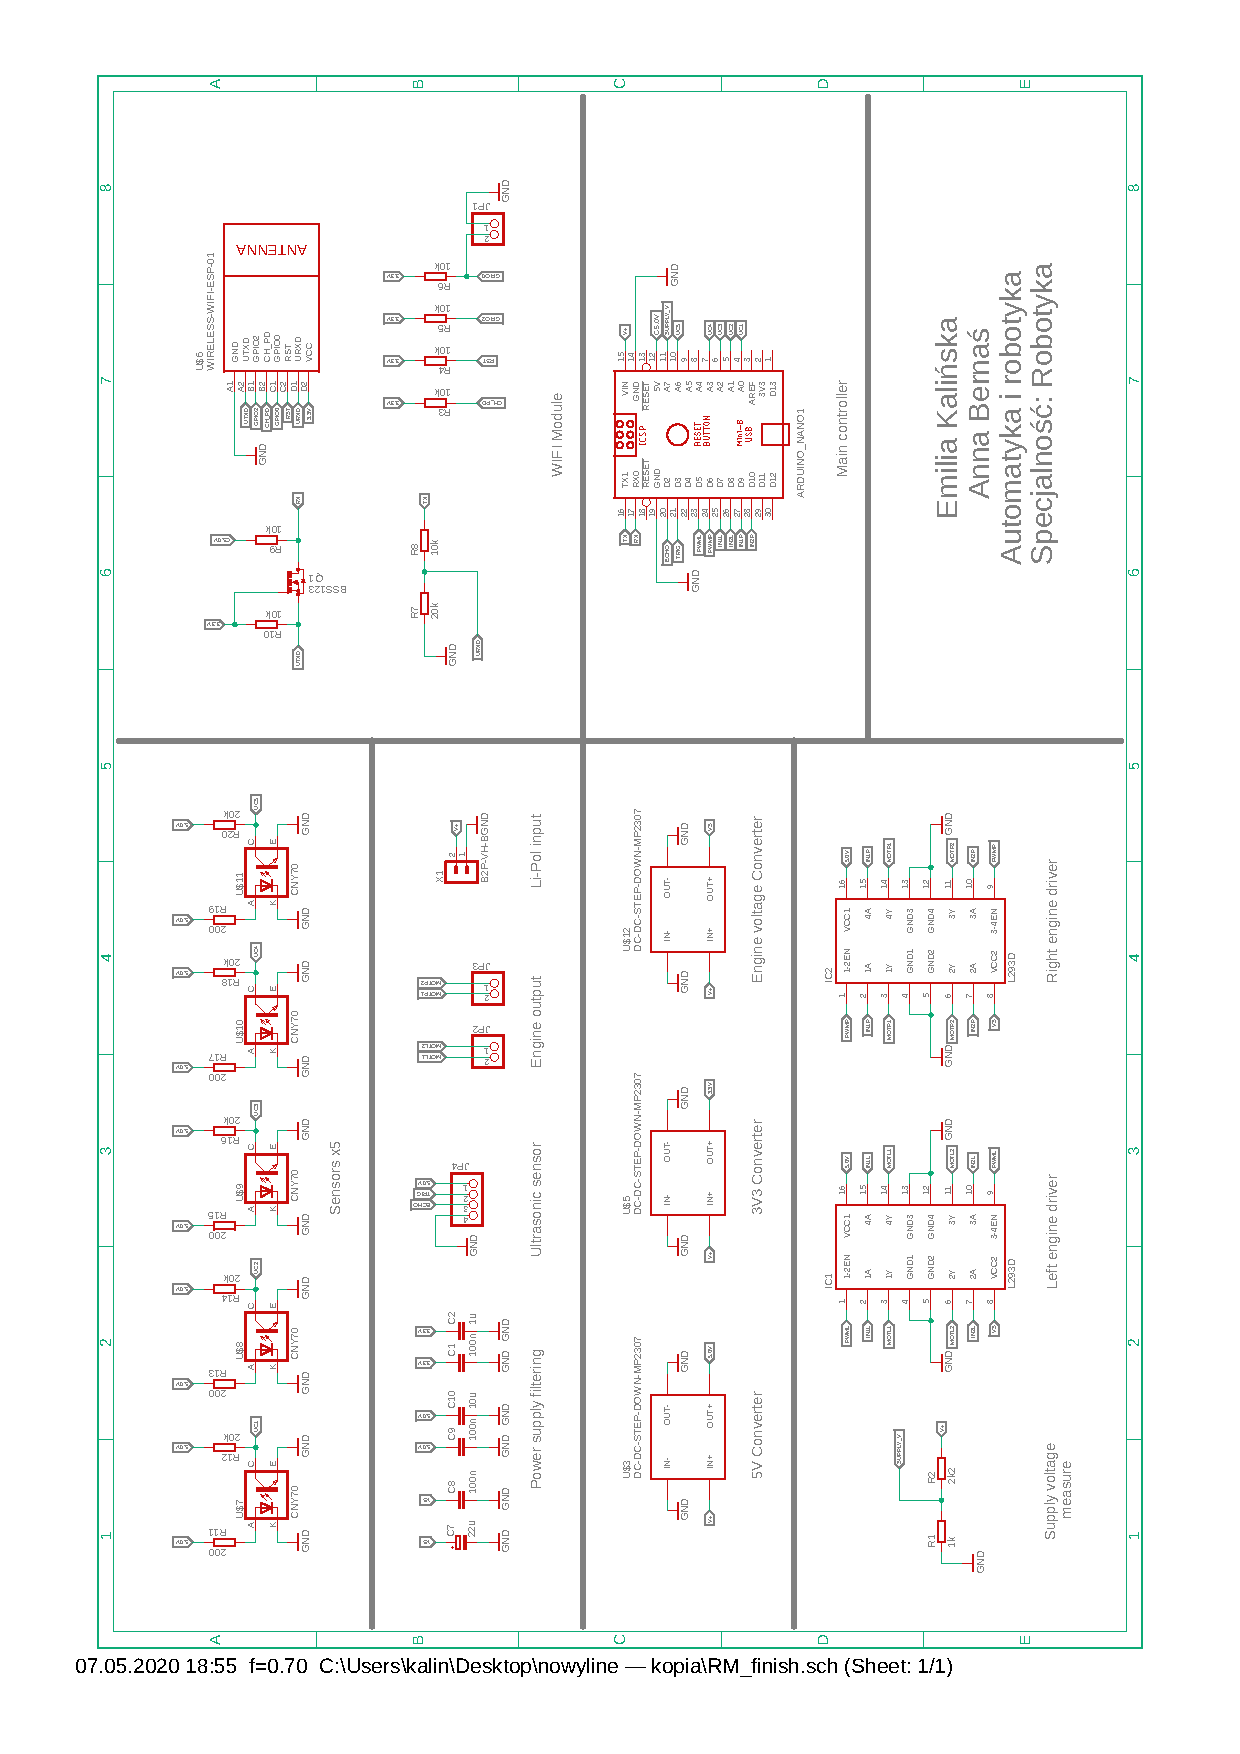
\includepdf[page={1}]{RM_schemat.pdf}
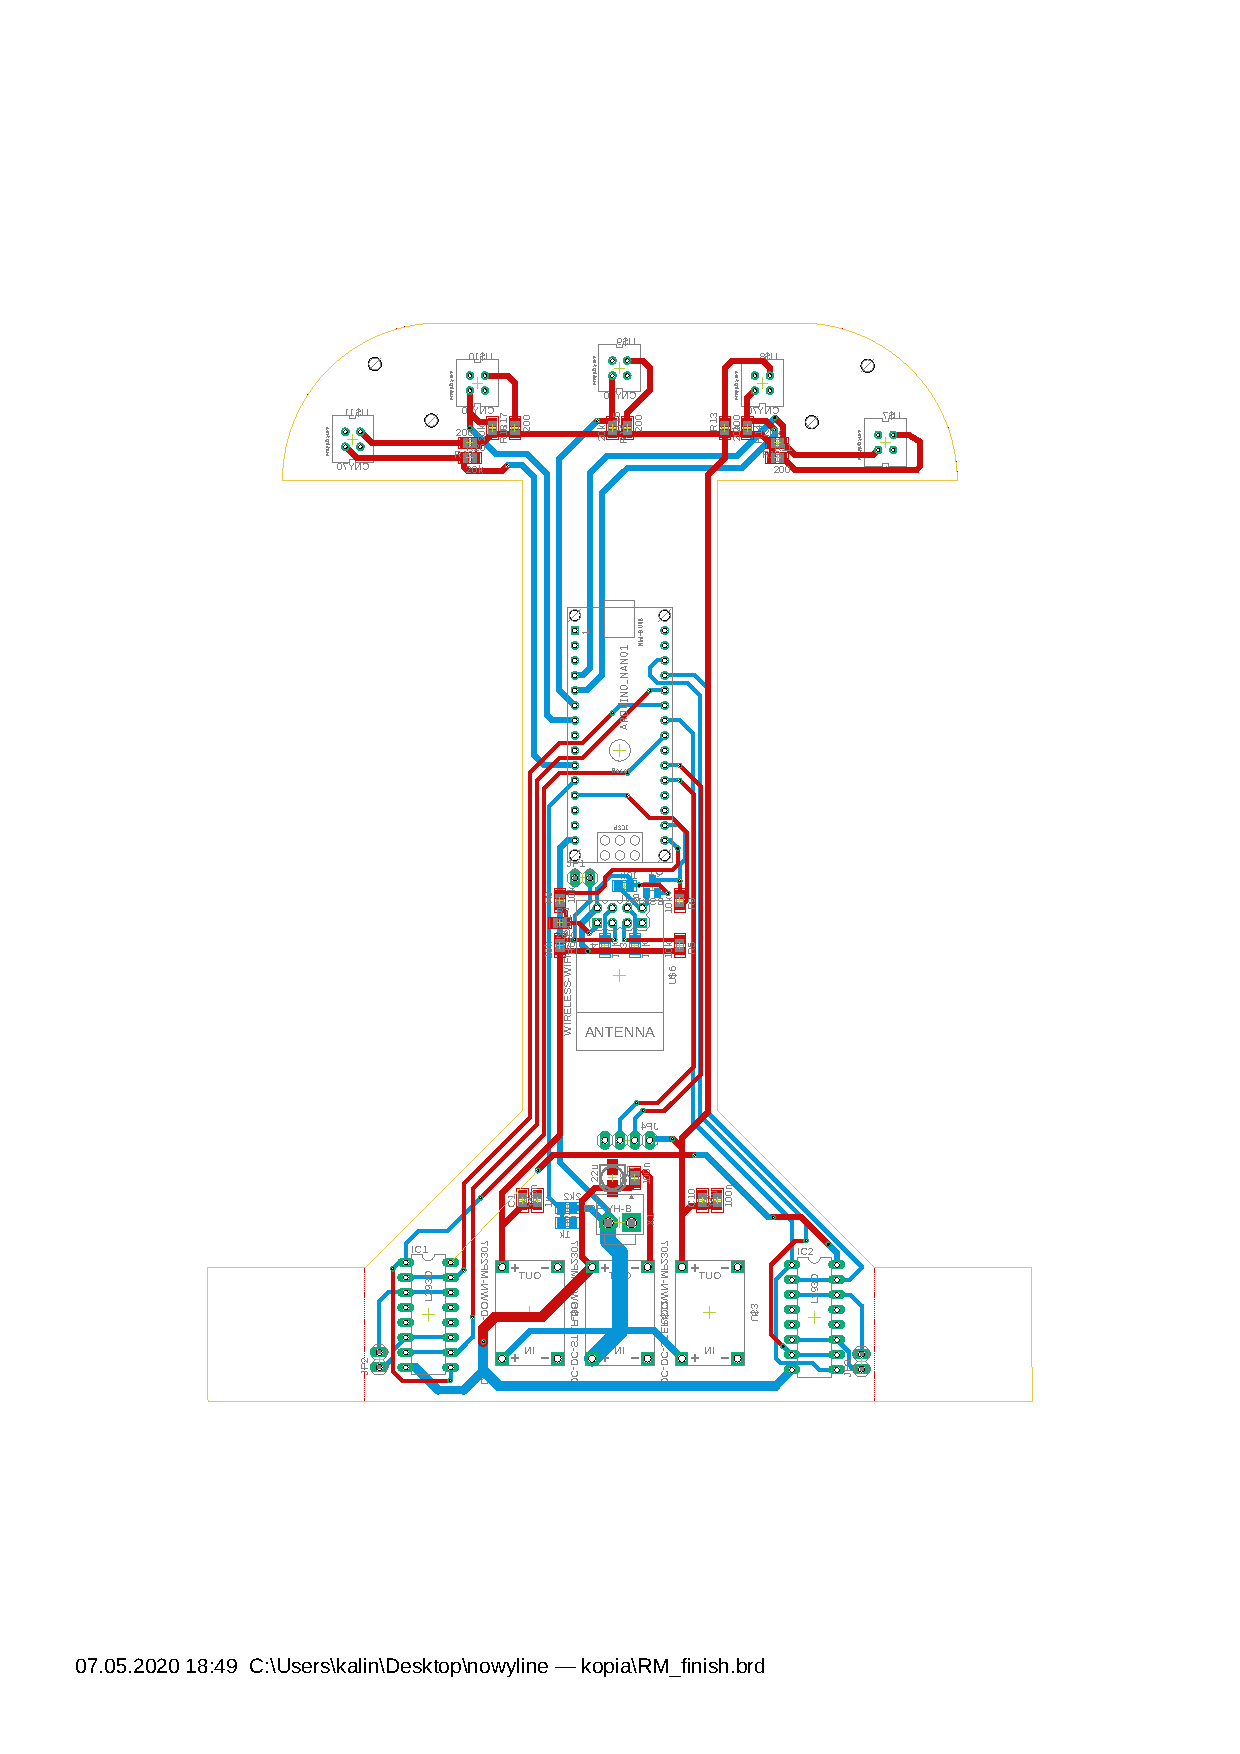
\includepdf[page={1}]{RM_finish.pdf}
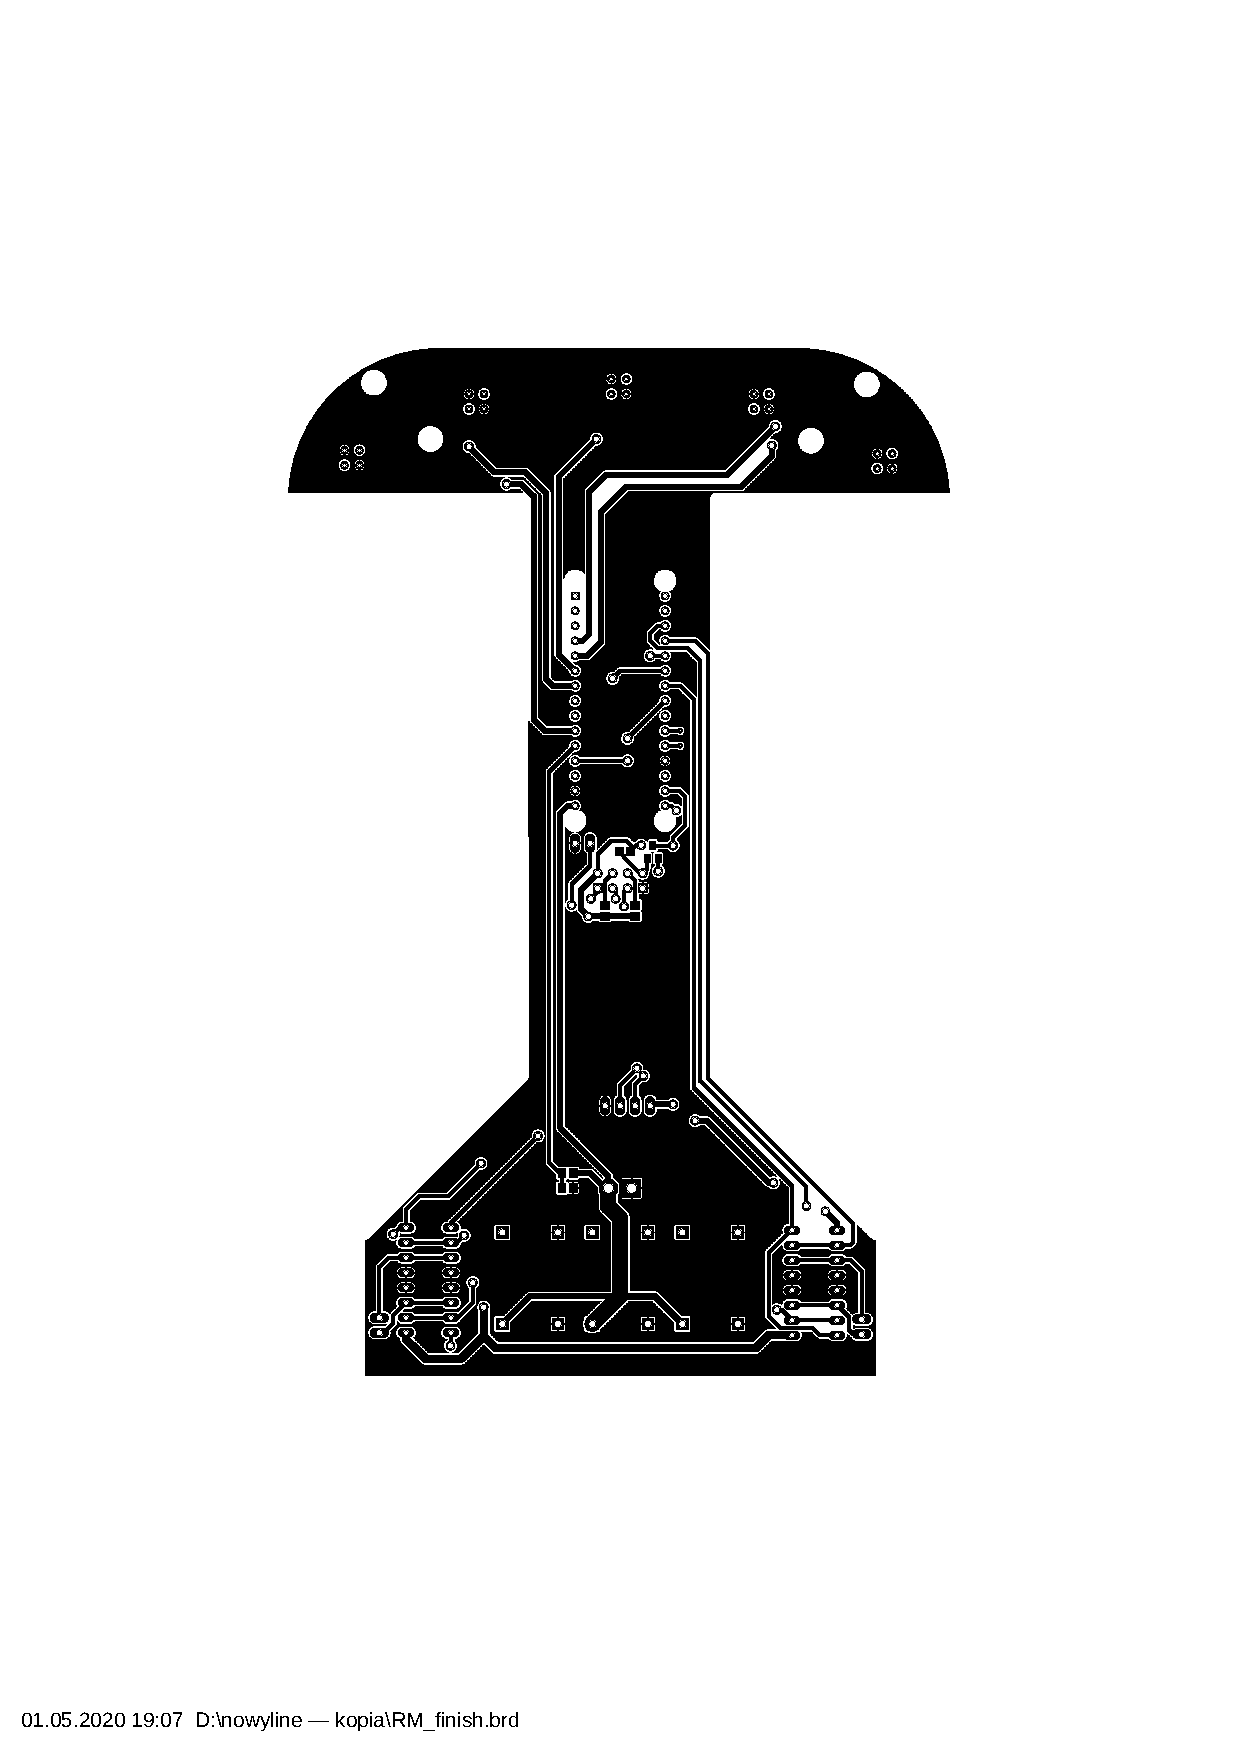
\includepdf[page={1}]{bottom.pdf}
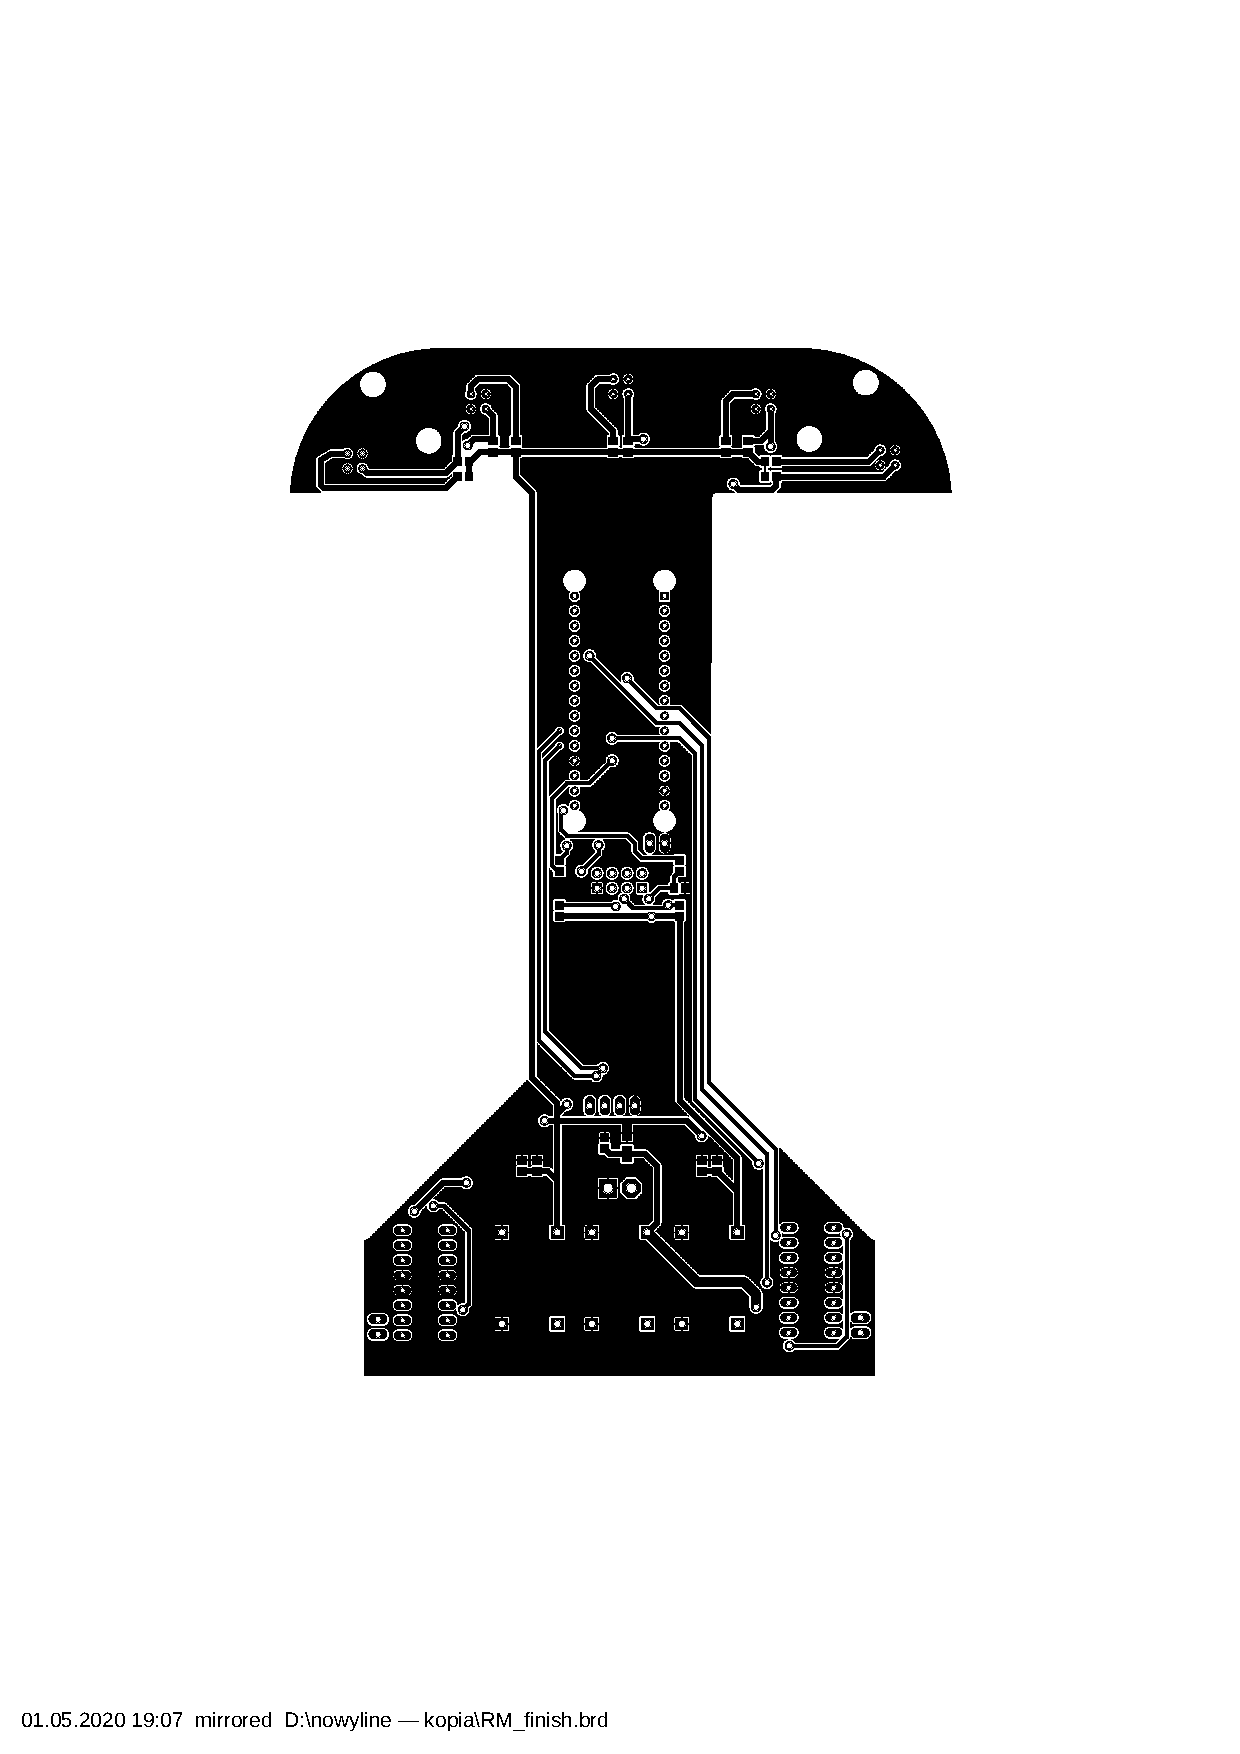
\includepdf[page={1}]{top.pdf}

%Obecne w dokumencie do etapu II oraz III
\section{Konstrukcja mechaniczna}

Płytka PCB o grubości 1,6mm będzie podwoziem robota. Ma ona kształt klasyczny dla robotów typu linefollower. Napęd będzie zrealizowany na tylną oś a na przedniej zostaną zamontowane kulki podporowe. Do zamontowania silników zostaną użyte przeznaczone im mocowania (POLOLU-989). Użyte koła to POLOLU 1453 40x7mm. Rozkład ciężkości będzie skupiony w tylnej częsći robota - będą w niej przymocowane silniki, przetwornice oraz akumulator.


%Obecne w dokumencie do etapu II oraz III (jeśli coś zostało niezrealizowane)
\section{Zadania niezrealizowane}

Robot nie został do końca złożony, aczkolwiek w założeniach wstępnych grupa zastrzegła sobie możliwość przesunięcia tego zadania na kolejny etap. Wykonanie płytki miało zostać zlecone firmie, która z powodu COVID-19 wstrzymała wysyłki do Polski. Po skontaktowaniu się z innymi przedsiębiorstwami zajmującymi się tą dziedziną, które proponowały ceny znacznie przekraczające budżet, grupa zdecydowała się na samodzielne wytrawienie płytki. Jeden z etapów wytrawiania został zaprezentowany na rysunku \ref{fig:wytrawianie}. Z tego powodu zajęło to znacznie więcej czasu niż było przewidywane. Na kolejny etap zostały przeniesione następujące czynności:
\begin{itemize}
    \item nastawienie oraz wlutowanie przetwornic,
    \item montaż silników, kół oraz kulek podporowych,
    \item wyfrezowanie płytki w odpowiedni kształt,
    \item odpowiednie zamocowanie akumulatora.
    
\end{itemize}

\begin{figure}[H]
    \centering
    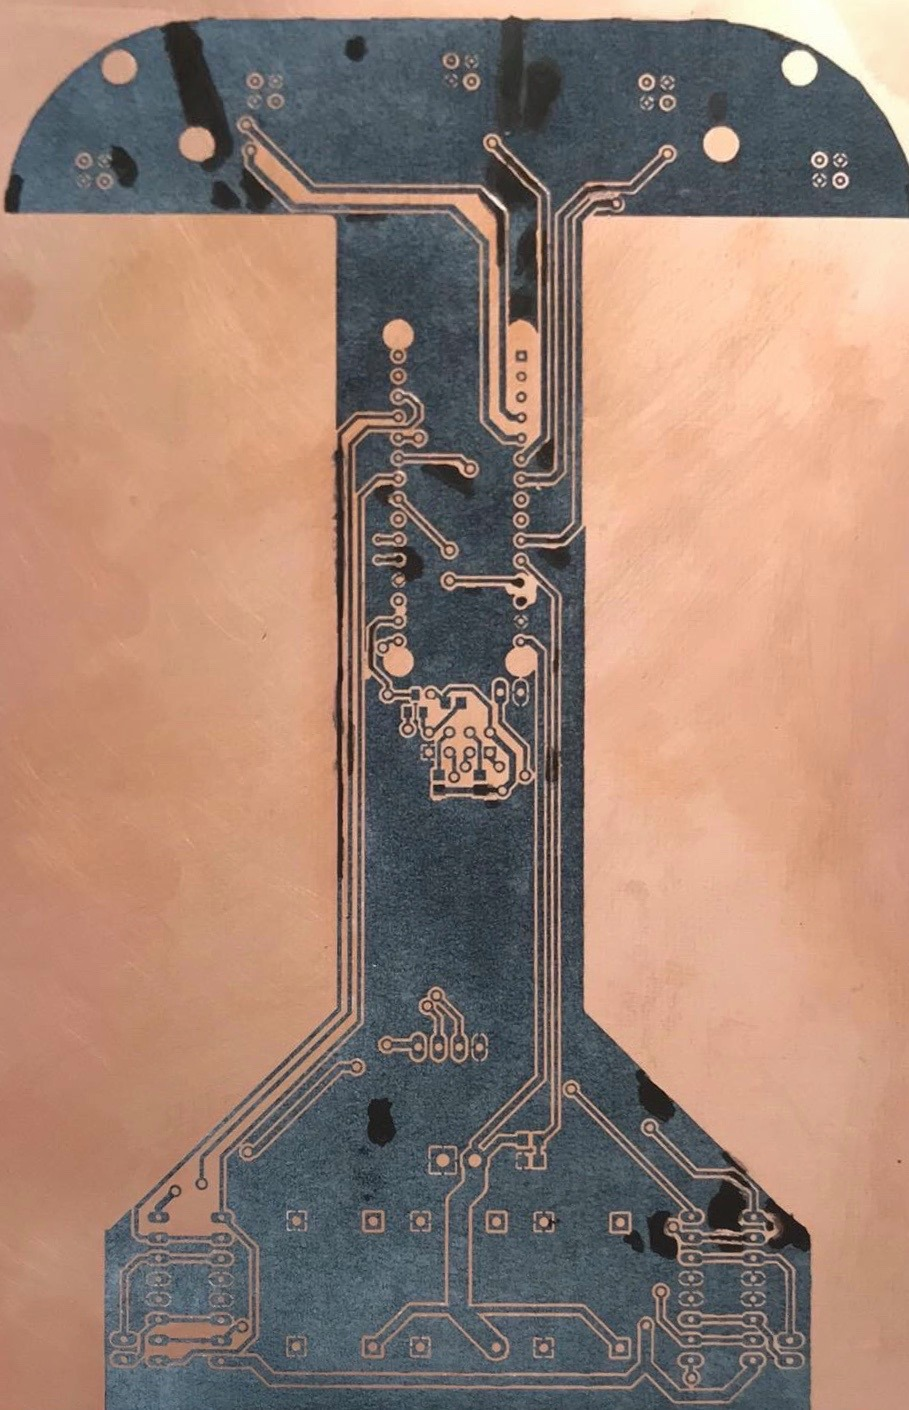
\includegraphics[width = 0.5\textwidth]{wytrawianie.jpg}
    \caption{Samodzielne wytrawianie płytki}
    \label{fig:wytrawianie}
\end{figure}

%Obecne we wszystkich dokumentach
\section{Podsumowanie}
Z powodów niezależnych od członków zespołu w tym etapie wykonano więcej zadań oraz poświęcono więcej czasu niż zakładano w harmonogramie. Pomimo trudności, które się pojawiły, grupa zakończyła etap związany bezpośrednio z elektroniką i mechaniką. Do wykonania zostały drobne czynności montażowe, które nie powinny znacząco wpłynąć na czas realizacji etapu III. Obecny stan projektu zaprezentowany jest na zdjęciach \ref{fig:efekty}.





\begin{figure}[H]
   \centering
    \subfigure[Góra płytki]{
    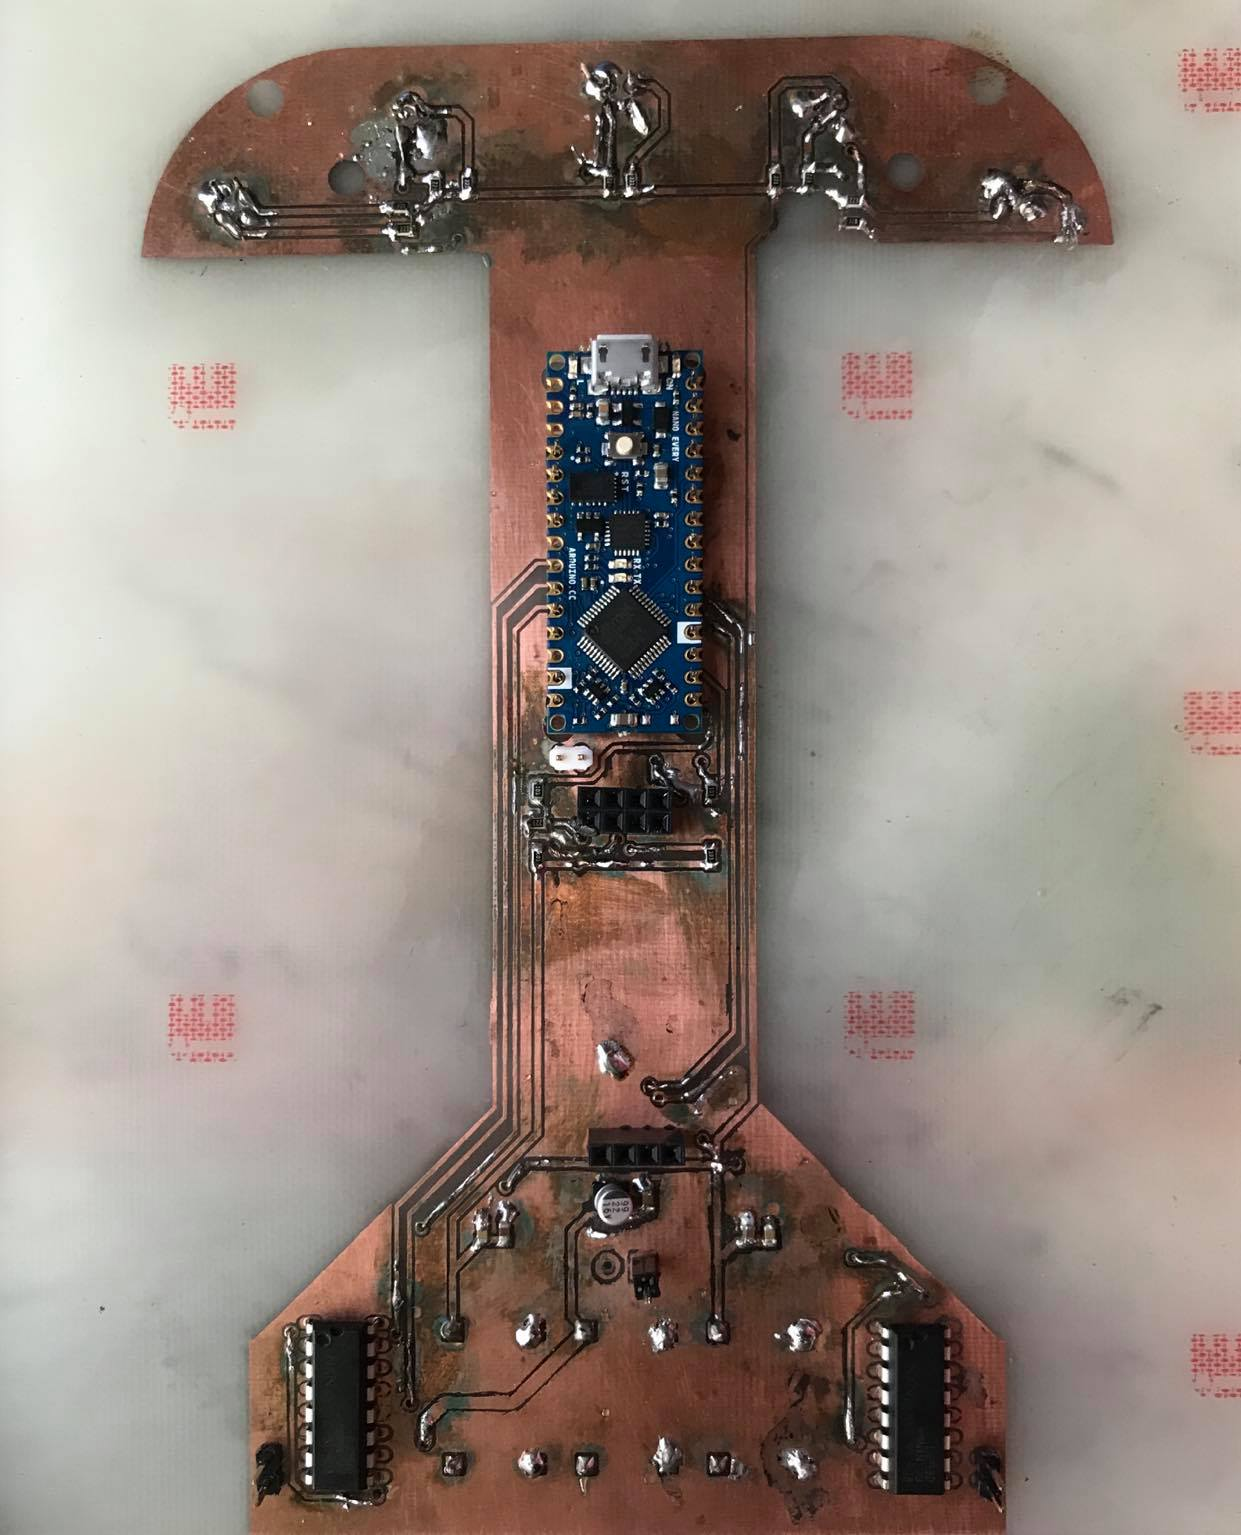
\includegraphics[height=0.5\textwidth]{topLine.jpg}
    \label{subfig:top}}
    \quad
    \subfigure[Dół płytki]{
    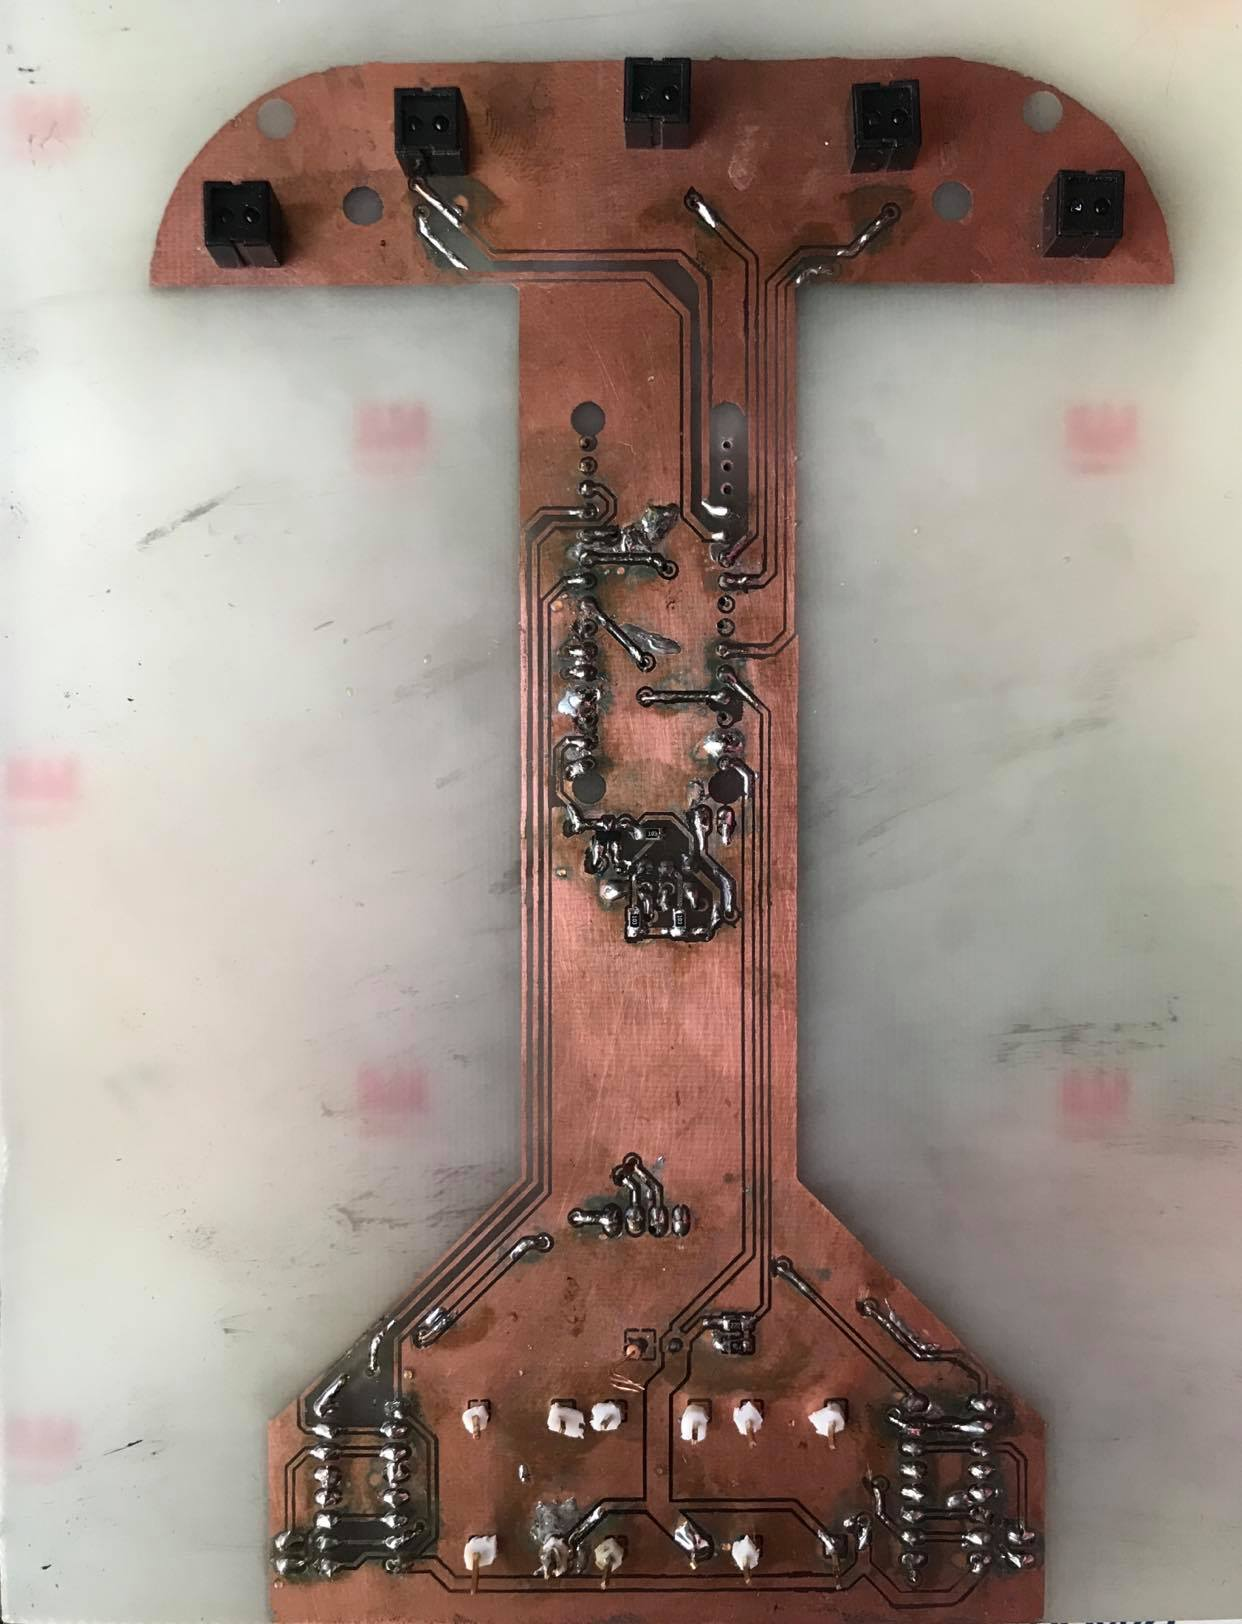
\includegraphics[height=0.5\textwidth]{bottomLine.jpg}
    \label{subfig:bot}}

    \caption{Uzyskane efekty}
    \label{fig:efekty}
   
\end{figure}
\newpage

\addcontentsline{toc}{section}{Bibilografia}
\bibliography{bibliografia}{}
\bibliographystyle{plabbrv}
\nocite{ksiazka1}
\nocite{ksiazka2}
\nocite{gazetka}

\nocite{dok1}
\nocite{dok2}
\nocite{dok3}
\nocite{dok4}
\nocite{dok5}
\nocite{dok6}



\end{document}







































